\documentclass[a4paper, 11pt]{article}

\usepackage[left=1.5cm, right=1.5cm, top=2cm, bottom=2cm]{geometry}

\usepackage[utf8]{inputenc}
\usepackage[T1]{fontenc}
\usepackage[english]{babel}  
\usepackage{lmodern}

\usepackage{amsmath, amsthm, amssymb}
\usepackage{mathtools}
\usepackage{dsfont}
\usepackage{stmaryrd}
\usepackage{breqn}

\newtheorem{innercustomgeneric}{\customgenericname}
\providecommand{\customgenericname}{}
\newcommand{\newcustomtheorem}[2]{%
  \newenvironment{#1}[1]
  {%
   \renewcommand\customgenericname{#2}%
   \renewcommand\theinnercustomgeneric{##1}%
   \innercustomgeneric}
  {\endinnercustomgeneric}
}

\newcustomtheorem{thm}{Theorem}
\newcustomtheorem{lem}{Lemma}
\newcustomtheorem{cor}{Corollary}
\newcustomtheorem{deftn}{Definition}
\newcustomtheorem{prop}{Proposition}
\newcustomtheorem{remark}{Remark}

\DeclareMathOperator*{\argmin}{argmin} 
\DeclareMathOperator*{\argmax}{argmax}
\DeclareMathOperator*{\essinf}{ess\ inf}
\DeclareMathOperator*{\esssup}{ess\ sup} 

\renewcommand{\thesection}{\Roman{section}} 

\begin{document}
\title{Hermite Polynomials snakes}
\author{Yoann Pradat}
\maketitle
\tableofcontents

\section{Translation of Schoenberg's 1973 paper}

The following is simply a reminder of some of the results found by I.J Schoenberg in his paper \emph{Cardinal 
Interpolation and Spline Functions. III Cardinal Hermite interpolation}. Let's reintroduce notations of the article and 
make somehow more explicits what the objects they encode are. \\

Let $r$ and $m$ be positive integers that satisfy $r \leq m$. The set of cardinal splines of order $2m$ with knot 
multiplicity $r$ is denoted by $S_{2m,r}$. Note that using De Boor's notations for splines set we have the following

\begin{equation}
  S_{2m,r} = \$_{2m, \mathbb{Z}_r} = \Pi_{< 2m, \mathbb{Z}, 2m-r}
\end{equation}

where $\mathbb{Z}_{3}$ denotes the sequence of knots $(\dots, -1,\dots,-1, 0, \dots, 0, 1, \dots, 1, \dots)$ that is 
integers with multiplicity $r$. It is clear from these notations that $S_{2m, r} \subset \mathcal{C}^{2m-r-1}$. 

\begin{thm}{1}
  Let $S$ be either of the vector spaces $\mathcal{L}_{p,r}, F_{\gamma,r}$ with $\gamma \geq 0$, $p \in \mathbb{N}^*$.  
  Provided a solution to C.H.I.P $\left( y_{\nu}, \dots,  y_{\nu}^{(r-1)}, S_{2m,r} \cap S \right)$ exists, it is 
  uniquely given by
  \begin{equation}
    \forall x \in \mathbb{R} \qquad S(x) = \sum_{\nu = - \infty}^{\infty} y_{\nu} L_0(x-\nu) + \cdots + y_{\nu}^{(r-1)} 
    L_{r-1}(x-\nu)
  \end{equation}
\end{thm}

In order to specify a usable model for active contours it remains to determine explicit expressions for the basis 
functions $L_0, \dots, L_{r-1}$. In the article they are determined by solving a set of $2m-r$ linear equations. This 
system is obtained by considering separately the function $L_s$ on $[1, \infty)$ and $[0,1]$. Note that specifying the 
function on both these intervals completely determine $L_s$ as the latter is even (if $s$ is even) or odd (if $s$ is 
odd). \\  

On $[1,\infty)$, $L_s$ can be decomposed into 

\begin{equation*}
  L_s = \sum_{j=1}^{m-r} c_j S_j
\end{equation*}

where ${(c_j)}_{j=1}^{m-r}$ are $(m-r)$ unknown coefficients to be determined and $S_j$ are the eigensplines for the 
first $m-r$ “eigenvalues” $\lambda_j$, solutions to $|\Delta_{r,d}(\lambda)|=0$. \\

On $[0,1]$, $L_s$ is given by a polynomial $P$ of order $2m$ that takes a specific form according to the parities of $s$ 
and $r$ (we refer to equations (7.13) and (7.14)) in the article. This polynomial introduces $m$ unknown coefficients 
${(a_j)}_{j=1}^{m}$. To determine a total of $m + m-r = 2m-r$ unknown coefficients we make use of the $2m-r$ equality 
conditions at 1 $P^{(\rho)}(1) = L_s^{(\rho)}(1)$. We end up of a system of $2m-r$ equations for $2m-r$ unknowns that 
can be solved exactly provided the matrix of the system is non singular. Schoenberg proves with a very nice argument 
that the matrix of the system is always non singular. \\

\subsection{General case $m=r$}\label{subsec:general_m_r}

In the case $m=r$, splines $L_s$ ($s=0, \dots, r-1$) vanish outside $[-1,1]$ and therefore give rise to a local 
interpolation scheme as given below for the case of periodic sequences. Let renote $\phi_s = L_{s-1}$ those  elements of 
$S_{2r, r}$ with support in $[-1,1]$ and that together satisfy Hermite interpolation conditions.

\begin{cor}{1}
  Given $r$ $M$-periodic sequences  ${(r[k], \dots, r^{(r-1)}[k])}_{k \in \mathbb{Z}}$ in $\mathbb{R}^d$, there exists a 
  unique spline curve of order $2r$ whose value and derivatives agree with the sequence of coefficients at integers 
  locations.  This spline curve and its derivatives are everywhere bounded and take the form for $t \in \mathbb{R}$
  
  \begin{align}
    r(t) &= \sum_{k \in \mathbb{Z}} \sum_{l=1}^r r^{(l-1)}[k] \phi_l(t-k) \\
    &= \sum_{k=0}^{M-1} \sum_{l=1}^r  r^{(l-1)}[k] \phi_{l, per}(t-k)
  \end{align}
  where $\phi_{l, per} = \sum_{k \in \mathbb{Z}} \phi_l(.-Mk)$

\end{cor}

In case the sequences are not periodic but have a finite number of non-zero entries, say $M$, we can similarly restrict 
the infinite sum to $M$ elements withouth periodizing the basis functions

\begin{cor}{2}
  Given $r$ sequences  ${(r[k], \dots, r^{(r-1)}[k])}_{k \in \mathbb{Z}}$ in $\mathbb{R}^d$ that vanish outside 
  $\llbracket 0, M \rrbracket$, there exists a unique spline curve of order $2r$ whose value and derivatives agree with 
  the sequence of coefficients at integers locations.  This spline curve and its derivatives have compact support and 
  take the form for $t \in \mathbb{R}$
  
  \begin{align}
    r(t) &= \sum_{k \in \mathbb{Z}} \sum_{l=1}^r r^{(l-1)}[k] \phi_l(t-k) \\
    &= \sum_{k=0}^{M-1} \sum_{l=1}^r  r^{(l-1)}[k] \phi_{l}(t-k)
  \end{align}
\end{cor}


\subsection{Case $m=r=3$}

In the case $m=r=3$, $L_0, L_1, L_2$ are 0 on $[1, \infty)$ and on $[0,1]$ are given by 

\begin{align}
  L_0(x) &= 1 + a_1 x^3 + a_2 x^4 + a_3 x^5 \\
  L_1(x) &= x + a_1 x^3 + a_2 x^4 + a_3 x^5 \\
  L_2(x) &= \frac{1}{2}x^2 + a_1 x^3 + a_2 x^4 + a_3 x^5
\end{align}

where the coefficients for each generator are unrelated. Note that $L_s$ have finite support \emph{because} $m=r$. If 
that was not the case the term $\displaystyle \sum_{j=1}^{m-r} c_j S_j$ may not be 0 and therefore $L_s$ would be non 
zero on $[1, \infty)$! Can it happen though that $m > r$ and ${(c_j)}_{j=1}^{m-r}$ are 0? To determine the coefficients 
above we need to solve independently for each generator the 3 equations $P^{(\rho)}(1) = 0$. This leads to the following 
systems

\begin{equation*}
  \left\{
  \begin{array}{r @{{}={}} r}
    a_1 + a_2  + a_3 & -1 \\
    3a_1 + 4a_2 + 5a_3 & 0 \\
    3a_1 + 6a_2  + 10a_3 & 0\\
  \end{array}
  \right.
  \hfill
  \left\{
  \begin{array}{r @{{}={}} r}
    a_1 + a_2  + a_3 & -1 \\
    3a_1 + 4a_2 + 5a_3 & -1 \\
    3a_1 + 6a_2  + 10a_3 & 0\\
  \end{array}
  \right.
  \hfill
  \left\{
  \begin{array}{r @{{}={}} r}
    a_1 + a_2  + a_3 & -\frac{1}{2} \\
    3a_1 + 4a_2 + 5a_3 & -1 \\
    3a_1 + 6a_2  + 10a_3 & -\frac{1}{2} \\
  \end{array}
  \right.
\end{equation*}

\section{The resulting snake scheme for $m=r=3$}

\subsection{Generating functions}

\begin{figure}[!h]
  \centering
  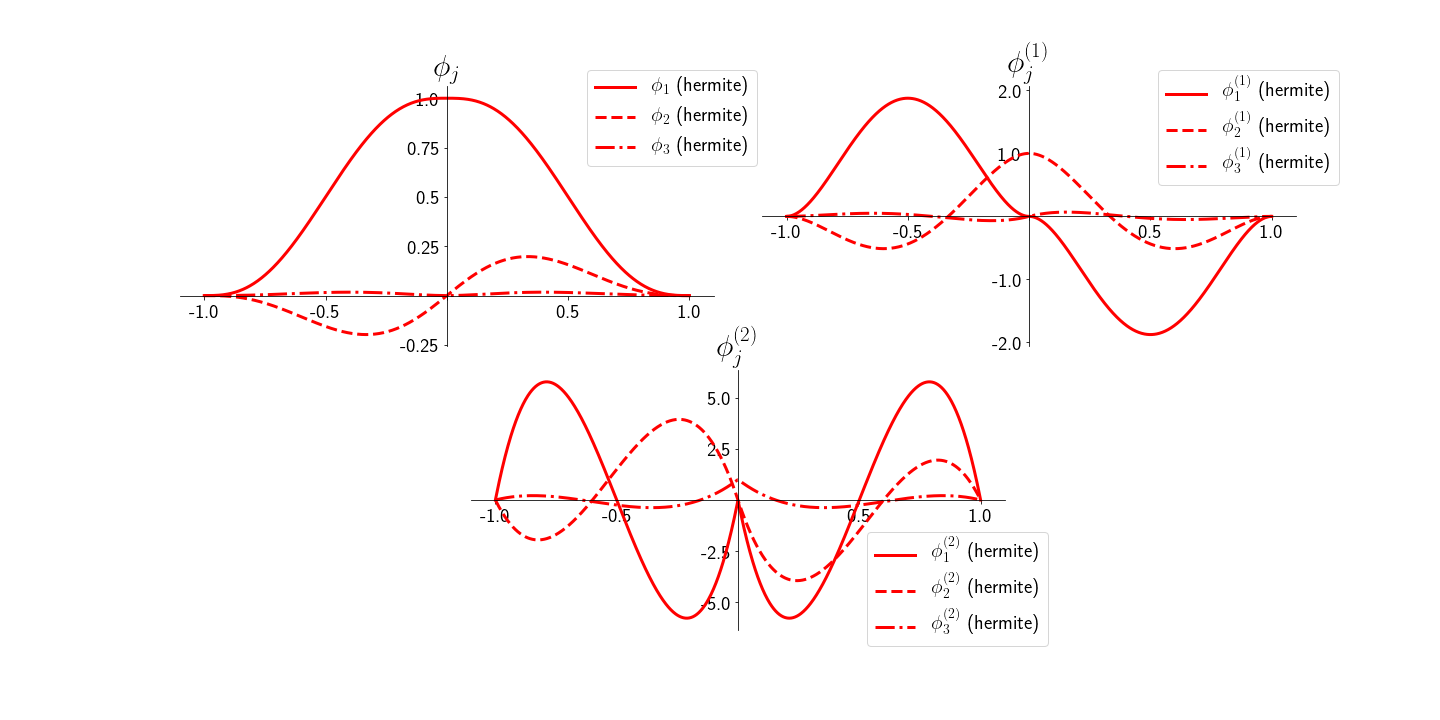
\includegraphics[width=\textwidth]{basis.png}
  \caption{Generators for C.H.I.P with $m=r=3$}\label{fig:basis}
\end{figure}


Solving the linear systems written in the previous section yields explicit formulas for the Schoenberg basis generators 
$L_0, L_1, L_2$, that we rename $\phi_1, \phi_2, \phi_3$ in accordance with modern notations (see V. Uhlmann 
\emph{Hermite Snakes with Controls of Tangents}). The formulas are the following. 

\begin{align}
  \phi_1(x) &= \begin{dcases} 
    1 - 10 x^3 + 15 x^4 - 6 x^5 & \text{if } 0 \leq x \leq 1  \\
    1 + 10 x^3 + 15 x^4 + 6 x^5 & \text{if } -1 \leq x < 0 \\
  \end{dcases} \\
  \phi_2(x) &= \begin{dcases}
    x - 6 x^3 + 8 x^4 - 3 x^5 & \text{if } 0 \leq x \leq 1  \\
    x - 6 x^3 - 8 x^4 - 3 x^5 & \text{if } -1 \leq x < 0 \\
  \end{dcases} \\
  \phi_3(x) &= \begin{dcases}
    0.5 x^2 - 1.5 x^3 + 1.5 x^4 - 0.5 x^5 & \text{if } 0 \leq x \leq 1  \\
    0.5 x^2 + 1.5 x^3 + 1.5 x^4 + 0.5 x^5 & \text{if } -1 \leq x < 0 \\
  \end{dcases}
\end{align}

In figure~\ref{fig:basis} are displayed the values of these functions as well as their two first derivatives. As 
mentioned in the previous section, the generators $L_s$ are elements of $S_{2m, r}=S_{6,3}$ which is a subset of 
$\mathcal{C}^{2m-r-1} = C^{2}$. It is apparent in the figure that these functions have continuous derivatives up to 
order 2 but that higher order derivatives do not exist in neighborhoods of $-1, 0$ and $1$.

\subsection{Closed planar curves or “contours”}

Consider a positive integer $M$ and an \textbf{$M$-periodic parametrized closed curve} $r: \mathbb{R} \to \mathbb{R}^2$ 
for which we have local derivatives up to order 2 at $M$ location sites regularly spaced that is we know ${(r[k], r'[k], 
r''[k])}_{k=0}^{M-1}$. 

\begin{cor}{3}
  Given $M$ periodic sequences  ${(r[k], r'[k], r''[k])}_{k \in \mathbb{Z}}$ in $\mathbb{R}^2$, there exists a unique 
  spline curve of order $6$ whose value and derivatives agree with the sequence of coefficients at integers locations.  
  This spline curve and its derivatives are everywhere bounded and take the form for $t \in \mathbb{R}$

\begin{align}
  r(t) &= \sum_{k \in \mathbb{Z}} r[k] \phi_1(t-k) + r'[k] \phi_2(t-k) + r''[k] \phi_3(t-k) \\
  &= \sum_{k=0}^{M-1} r[k] \phi_{1, per}(t-k) + r'[k] \phi_{2, per}(t-k) + r''[k] \phi_{3, per}(t-k) 
  \label{eq:curve_nno}
\end{align}

\end{cor}

\begin{proof}
As the sequence of coefficients ${(r[k], r'[k], r''[k])}_{k \in \mathbb{Z}}$  are in $Y_{\gamma, r} = Y_{0, 3}$ (i.e 
they are bounded), application of Schoenberg's theorem 1 yields existence and unicity of an interpolating function in 
$S_{6,3} \cap F_{0, 3}$. Application of theorem 4 then leads to the explicit formulation given above.
\end{proof}

\begin{remark}{1} It is convenient to normalize the continuous parameter to the $[0,1]$ interval as is usual in the 
  implementations.  For that let the renormalized curve $s(t) = r(Mt)$ for $t \in [0,1]$. Note that this completely 
  describes the curve as it is enough to describe the curve $r$ on $[0,M]$. Differentiating this equality twice yields 
  $r[k] = s[\frac{k}{M}], r'[k] = \frac{1}{M} s'[\frac{k}{M}], r''[k] = \frac{1}{M^2} s''[\frac{k}{M}]$. Therefore 
  equation (\ref{eq:curve_nno}) is rewritten for $t \in [0,1]$

\begin{equation}
  \label{eq:ccurve_no}
  s(t) = \sum_{k=0}^{M-1} s[\frac{k}{M}] \phi_{1, per}(Mt-k) + \frac{1}{M} s'[\frac{k}{M}] \phi_{2, per}(Mt-k) + 
  \frac{1}{M^2} s''[\frac{k}{M}] \phi_{3, per}(Mt-k)
\end{equation}

\end{remark}

In the rest of this document we will reuse the notation $r$ for the normalized curve and won't make use of the notation 
$s$ anymore. Equation (\ref{eq:ccurve_no}) is the \textbf{mathematical representation of a planar curve} and we call it 
“snake” or “active contour”. By playing with the coefficients we can capture a wide variety of contours that arise from 
closed objects in 2D images like cells membrane in a bioimage. 

\subsection{Open planar curves}

Consider again a positive integer $M$ and a \textbf{parametrized open curve} $r: \mathbb{R} \to \mathbb{R}^2$ for which 
we have local derivatives up to order 2 at $M$ location sites regularly spaced that is we know ${(r[k], r'[k], 
r''[k])}_{k=0}^{M-1}$. By “open” we mean a curve that is not periodic.  

\begin{cor}{4}
  Given biinfinite sequences of coefficients $(\dots, 0, r[0], \dots, r[M-1], 0, \dots)$, $(\dots, 0, r'[0], \dots, 
  r'[M-1], 0, \dots)$, $(\dots, 0, r''[0], \dots, r''[M-1], 0, \dots)$ in $\mathbb{R}^2$, there exists a unique spline 
  curve of order $6$ whose value and derivatives agree with the sequence of coefficients at integers locations. This 
  spline curve and its derivatives have compact support and take the form for $t \in \mathbb{R}$

  \begin{align*}
    r(t) &= \sum_{k \in \mathbb{Z}} r[k] \phi_1(t-k) + r'[k] \phi_2(t-k) + r''[k] \phi_3(t-k) \\
    &= \sum_{k=0}^{M-1} r[k] \phi_{1}(t-k) + r'[k] \phi_{2}(t-k) + r''[k] \phi_{3}(t-k)
  \end{align*}
\end{cor}

\begin{proof}
  This result is again a simple application of theorem 1 and 4 given in Schoenberg's paper of 1981.
\end{proof}

\begin{remark}{2}
  In this setting we are only interested in the curve lying between our coefficients that is the interpolated points 
  with continuous parameter in the interval $[0, M-1]$  The normalization factor is therefore $M-1$ and the renormalized 
  open curve $r(t) = r((M-1)t)$ takes the form

  \begin{equation}
    \label{eq:ocurve_no}
    r(t) = \sum_{k=0}^{M-1} r[\frac{k}{M-1}] \phi_{1}((M-1)t-k) + r'[\frac{k}{M-1}] \frac{\phi_{2}((M-1)t-k)}{M-1} + 
  r''[\frac{k}{M-1}] \frac{\phi_{3}((M-1)t-k)}{{(M-1)}^2} \end{equation}
\end{remark}

\subsection{Closed sphere-like surfaces}

In my research project we are interested in developing a mathematical methods for representing a certain type of 
surfaces with explicit control of local properties including first-order derivatives and curvature. As a consequence 
extension of the schemes given in equations (\ref{eq:ccurve_no}) and (\ref{eq:ocurve_no}) to tensor-product surfaces 
(that is surfaces parametrized by 2 continuous parameters in a way that each continuous parameter appear in separate 
functions) may be relevant for the questions we have. \\ 

Consider positives integers $M_1$ and $M_2$ and a \textbf{sphere-like parametrized} surface $\sigma: U \subseteq 
\mathbb{R}^2 \to \mathbb{R}^3$ with $U$ a subset (closed in our case) of the plane. By “sphere-like” we mean an object 
that can be described with closed curves on latitudes ($u$ varies while $v$ is fixed) and open curves on longitudes ($v$ 
varies while $u$ is fixed). Suppose we have local properties of the surface at $M_1\times(M_2+1)$ locations (counted 
with multiplicity as some locations may coalesce) on a regular grid. \\ 

\begin{cor}{5}
  Given the biinfinite sequences of coefficients ${(\partial^{i,j}\sigma(k,l))}_{k, l \in \mathbb{Z}^2, (i,j) \in 
  {\{0,1,2\}}^2}$ in $\mathbb{R}^3$, that are $M_1$ periodic in the first coordinate and vanish when the second 
  coordinate is outside $\llbracket 0, M_2 \rrbracket$, there exists a unique interpolating tensor-product spline curve 
  of order $6$ whose value and partial derivatives agree with the sequence of coefficients at the integers grid 
  locations.  This tensor-product spline curve and its derivatives are everywhere bounded and take the form for $(u,v) 
  \in [0,M_1]\times[0, M_2]$ (or equiv.
  $\mathbb{R}\times[0, M_2]$)

  \begin{equation}
    \sigma(u,v) = \sum_{k=0}^{M_1-1} \sum_{l=0}^{M_2} \sum_{i,j = 0}^2 \partial^{i,j} \sigma(k,l) \phi_{i+1, per}(u-k) 
    \phi_{j+1}(v-l)
  \end{equation}
\end{cor}

\begin{proof}
  This is a simple application of corollaries 1 and 2 given before.
\end{proof}

\begin{remark}{3}
  \begin{itemize}
    \item  Not all surfaces admit a tensor-product representation which limits the range of surfaces one can reach with 
      this kind of interpolation scheme. Tensor-product spline has not yet been defined and we just mention here  that 
      we call a tensor-product spline a map $f: U_1\times U_2 \subseteq \mathbb{R}^2 \to \mathbb{R}$ that can be written 
      as $f_1(u) \times f_2(v)$ with $f_1$ and $f_2$ each splines on $U_1$ and $U_2$ respectively.
    \item The continuity of the basis functions is automatically transferred to the each coordinate of the spline curve, 
      resulting in surfaces with parametrizations that are twice continuously differentiable. Is this preventing us from 
      representing surfaces with singular points as we would like to have? This question is crucial to our objective and 
      will be addressed later in more details.
    \item Normalizing each continuous parameter to the interval $[0,1]$ yields the following representation of the 
      surface (where we note again $\sigma$ the surface with normalized parameters)
      \begin{equation}
        \sigma(u,v) = \sum_{k=0}^{M_1-1} \sum_{l=0}^{M_2} \sum_{i,j = 0}^2 \frac{1}{M_1^i M_2^j} \partial^{i,j} 
        \sigma(\frac{k}{M_1}, \frac{l}{M_2}) \phi_{i+1, per}(M_1u-k) \phi_{j+1}(M_2v-l)
      \end{equation}
  \end{itemize}
\end{remark}

\section{Properties of the interpolation scheme}

\subsection{The Riesz-Schauder basis property}

\subsubsection{Definition}

\begin{deftn}{1}
  Let $\mathcal{H}$ be a Hilbert space over the field $\mathbb{K} = \mathbb{R}$ or $\mathbb{C}$ of real or complex 
  numbers. A basis ${\{\phi_k\}}_{k \in \mathbb{Z}}$ of $\mathcal{H}$ is said to be a Riesz-Schauder basis if there 
  exist positive constants $0 < m \leq M$ such that
  \begin{equation}
    \forall c \in l_2(\mathbb{Z}) (\subset \mathbb{K}^{\mathbb{Z}})  \qquad m {\|c\|}_{l_2}^2 \leq {\| \sum_{k \in 
    \mathbb{Z}} c_k \phi_k \|}_{\mathcal{H}}^2 \leq M {\|c\|}_{l_2}^2
  \end{equation}
\end{deftn}

Let $n$ be a positive integer, $f, g$ functions $\mathbb{R}^n \to \mathbb{C}$. Define $\lambda$ the Lebesgue measure on 
$\mathbb{R}^n$ and the map 

\begin{equation*}
  \langle f,g\rangle = \int_{\mathbb{R}^n} f\bar{g} d\lambda
\end{equation*}

This map is an inner product on the vector space over $\mathbb{C}$ of all measurable functions for which $\langle f,f 
\rangle$ is finite (to be precise we consider quotient space so that its elements are equivalence classes for the 
relation that two functions are equivalent if they agree $\lambda$-a.e).  The latter, endowed with this inner product, 
is therefore a pre-Hilbert space.  It is a known result that this space is complete and therefore a Hilbert space.  It 
is usually denoted by $L_2(\mathbb{R}^n)$.  For an element $f$ of that space we denote $\hat{f}$ the extension (by 
density) to functions in $L_2(\mathbb{R}^n)$ of the Fourier transform as usually defined in mathematics textbooks over 
functions in $L_1(\mathbb{R}^n)$.

\subsubsection{Characterization in the Fourier domain}

\begin{thm}{2}
  In case the Hilbert space $\mathcal{H}$ is $L_2(\mathbb{R}^n)$ and $\phi \in \mathcal{H}$, the following statements 
  for some $0 < m \leq M$ are equivalent
  \begin{enumerate}
    \item $\forall c \in l_2(\mathbb{Z})$, $\displaystyle m {\|c\|}_{l_2}^2 \leq {\| \sum_{k \in \mathbb{Z}} c_k 
      \phi(.-k) \|}_{L_2}^2 \leq M {\|c\|}_{l_2}^2$
    \item $\displaystyle m \leq  \sum_{k \in \mathbb{Z}} {|\hat{\phi}(w+2k\pi)|}^2 \leq M$ a.e
  \end{enumerate}
  with obvious notations. In case any of the two statements holds, the subspace $\displaystyle V= \{ \sum_{k \in 
  \mathbb{Z}} c_k \phi(.-k) | c \in l_2(\mathbb{Z}) \}$ of $L_2(\mathbb{R}^n)$ is closed and thus a Hilbert space 
  itself, and $\{\phi(.-k)\}$ is a Riesz-Schauder basis.
\end{thm}

\begin{proof}This theorem is exactly theorem $2$ as given in A. Aldroubi, M. Unser, “Sampling procedures in function 
  spaces and asymptotic equivalence with Shannon’s sampling theory,” Numer. Funct. Anal. Optim., vol. 15, nos. 1–2, pp.  
  1–21, May 1994 and is proved there for the case $n=1$ but extension to domain of generic dimension is straightforward.
\end{proof}

For the needs of having this Riesz-Schauder basis property for vector-valued basis functions let's give an immediate 
corollary for that case. For that let's define the map $\langle \cdot, \cdot \rangle$ over functions $\mathbb{R}^n \to 
\mathbb{C}^m$ by 

\begin{equation*}
  \langle f,g\rangle = \sum_{i=1}^m \int_{\mathbb{R}^n} f_i\bar{g_i} d\lambda
\end{equation*}
  
with obvious notations.  This map defines an inner product and the space $L_2(\mathbb{R}^n, \mathbb{C}^m)$ of functions 
having finite norm as induced by this inner product is a Hilbert space.


\begin{thm}{3}\label{thm:multi}
  In case the Hilbert space $\mathcal{H}$ is $L_2(\mathbb{R}^n, \mathbb{C}^m)$ and $\phi \in \mathcal{H}$, the following 
  statements for some $0 < m \leq M$ are equivalent
  \begin{enumerate}
    \item $\forall c \in l_2(\mathbb{Z})$,  $\displaystyle m {\|c\|}_{l_2}^2 \leq {\| \sum_{k \in \mathbb{Z}} c_k 
      \phi(.-k) \|}_{L_2(\mathbb{R}^n, \mathbb{C}^m)}^2 \leq M {\|c\|}_{l_2}^2$
    \item $\displaystyle m \leq  \sum_{k \in \mathbb{Z}} \sum_{i=1}^m {|\hat{\phi_i}(w+2k\pi)|}^2 = \sum_{k \in 
      \mathbb{Z}} {\|\hat{\phi}(w+2k\pi)\|}_{2}^2  \leq M$
  \end{enumerate}
  with obvious notations. In case any of the two statements holds, the subspace $\displaystyle V= \{ \sum_{k \in 
  \mathbb{Z}} c_k \phi(.-k) | c \in l_2(\mathbb{Z}) \}$ of $L_2(\mathbb{R}^n, \mathbb{C}^m)$ is closed and thus a 
  Hilbert space itself, and $\{\phi(.-k)\}$ is a Riesz-Schauder basis.
\end{thm}

\subsubsection{Characterization from Gram matrix}

In cases where there are several generators, like the Hermite polynomial interpolation, one can characterize the 
property of Riesz-Schauder basis from the Gram-matrix of the set of generators $\{\phi_i(.-k)\}$. For that, let 
${\{\phi^i\}}_{i=1}^q$ be functions in a Hilbert space $\mathcal{H}$ and let $O$ be a unitary operator on $\mathcal{H}$ 
i.e $OO^* = O^*O = I$ (in our case of Hermite interpolation $O\phi = \phi(.-1)$). \\ 

Consider the subspace $\displaystyle V= \{  \sum_{k \in \mathbb{Z}} C(k) O^k\Phi = \sum_{k \in \mathbb{Z}} \sum_{i=1}^q 
c^i(k) O^k\phi^i  | c^1, \ldots, c^q \in l_2(\mathbb{Z})\}$. As seen before $V$ is a well-defined closed subspace of 
$\mathcal{H}$ if there exists constants $0 < m \leq M$ such that

\begin{equation}
  \forall C \in l_2^q(\mathbb{Z}) \quad  m {\|C\|}_{l_2^q}^2 \leq {\| \sum_{k \in \mathbb{Z}} C(k) O^k\Phi
  \|}_{\mathcal{H}}^2 \leq M {\|C\|}_{l_2^r}^2
\end{equation}

Note that the central term of the inequality above can be rewritten as

\begin{align*}
  \langle \sum_{k \in \mathbb{Z}} C(k) O^k\Phi, \sum_{l \in \mathbb{Z}} C(l) O^l\Phi \rangle & = \sum_{(k,l) \in 
  \mathbb{Z}^2} C(k) \langle O^k\Phi, O^l\Phi \rangle C(l)^* \\
  &=  \sum_{(k,l) \in \mathbb{Z}^2} C(k) A(l-k) C(l)^*
\end{align*}

where $A$ is a $q\times q$ matrix with elements $A_{i,j}(k) = \langle \phi^i, O^k\phi^j \rangle$. Now the above can be 
viewed as

\begin{equation*}
  \sum_{(k,l) \in \mathbb{Z}^2} C(k) A(l-k) C(l)^* = \sum_{i,j=1}^q \sum_{l \in \mathbb{Z}} (c^i * A_{i,j}) (l) {c^j}^* 
  (l)
\end{equation*}

Using Parseval's theorem for discrete time Fourier transform that is $\hat{c}(w) = \sum_{k \in \mathbb{Z}} c(k) 
e^{-jwk}$ or in $f$-notation $\hat{c}(f) = \sum_{k \in \mathbb{Z}} c(k) e^{-j2\pi fk}$ we have that

\begin{align*}
  \sum_{i,j=1}^q \sum_{l \in \mathbb{Z}} (c^i * A_{i,j}) (l) {c^j}^* (l) &= \sum_{i,j=1}^q \frac{1}{2\pi} 
  \int_{0}^{2\pi} \hat{c^i}(w) \hat{A}_{i,j}(w) \hat{c^j}^*(w) \frac{dw}{2\pi} \\
  &= \frac{1}{2\pi} \int_{0}^{2\pi} \hat{C}(w) \hat{A}(w) \hat{C}^*(w) \frac{dw}{2\pi} \\
  &= \int_{0}^{1} \hat{C}(f) \hat{A}(f) \hat{C}^*(f) df
\end{align*}

$\hat{A}(w)$ with elements $A_{i,j}(w) = \sum_{k \in \mathbb{Z}} \langle \phi^i, O^k \phi^j \rangle e^{-jwk}$ is called 
the \textbf{Gram matrix}. Now theorem 2.1 from 1996 paper by Adroubi \emph{Oblique Projections in Atomic Spaces} makes 
the link between $m,M$ constants characterizing Riesz-Schauder basis property and the minimum and maximum eigenvalue of 
the Gram matrix as follows

\begin{thm}{4}
  \label{thm:gram}
  The space $V$ is a well-defined closed subspace of $\mathcal{H}$ with Riesz-Schauder basis $\{O^k 
  \phi^i\}_{i=1,\dots,q, k \in \mathbb{Z}}$ if and only if the $q\times q$ Gram matrix $\hat{A}(w)$ is hermitian 
  positive for almost all $w$ and there exist two constants $0 < m \leq M$ such that
  \begin{equation}
    \label{eq:ess}
    m \leq \essinf_{w \in [-\pi, \pi]} \lambda_{min}(\hat{A}(w)) \leq \esssup_{w \in [-\pi, \pi]} 
  \lambda_{max}(\hat{A}(w)) \leq M \end{equation}
\end{thm}

\begin{proof} This is exactly theorem 2.1 as stated in the article mentioned and the proof is given there.
\end{proof}

\subsection{Riesz-Schauder basis for Hermite interpolation order $r$}

Let $r$ be a positive integer and $\phi_1, \ldots, \phi_r$ the elements of $S_{2r, r} \cap \mathcal{L}_{1,r}$ with 
support in $[-1,1]$ that satisfy Hermite interpolation conditions as introduced in subsection~\ref{subsec:general_m_r}.  
Consider a positive integer $d$ representing the dimension of the space in which the coefficients of the resulting 
scheme live i.e 

\begin{equation}
  \label{eq:Phi}
  V = \{ \sum_{k \in \mathbb{Z}} C(k) \Phi(.-k) | C \in l_2^{d\times r}(\mathbb{Z}) \}
\end{equation}

with $\Phi(.-k) = \begin{pmatrix} \phi_1 & \cdots & \phi_r \end{pmatrix}^T$, $C(k) =  \begin{pmatrix} c_1(k) & \cdots & 
c_r(k) \end{pmatrix}$ and $c_l \in l_2^d(\mathbb{Z})$. Note that $V$ is a subspace of $L_2(\mathbb{R}, \mathbb{R}^d)$.  
To state properly the Riesz-basis property we need to exhibit functions that are elements of $L_2(\mathbb{R}, 
\mathbb{R}^d)$. For that consider the functions $\phi_j e_i$ for $j=1, \ldots, r$, $i=1, \ldots, d$ with $(e_i)_{i=1}^d$ 
the canonical base of $\mathbb{R}^d$.  Then $V$ can be rewritten as

\begin{equation}
  V = \{ \sum_{k \in \mathbb{Z}} \sum_{j=1}^r \sum_{i=1}^d c_{j, i}(k) \phi_j(.-k)e_i | c \in l_2(\mathbb{Z}) \}
\end{equation}

which amounts to taking $\Phi(.-k) = \begin{pmatrix} \phi_1e_1 & \cdots, \phi_1 e_d & \cdots & \phi_r e_1 & \cdots & 
\phi_r e_d \end{pmatrix}^T$, $C(k) =  \begin{pmatrix} c_1(k) & \cdots & c_{rd}(k) \end{pmatrix}$ in notations of 
(\ref{eq:Phi}). Theorem~\ref{thm:riesz} shows that Riesz-Schauder basis property holds at any order $r$ for Hermite 
polynomial interpolation.

\begin{thm}{5}
  \label{thm:riesz}
  Let $r$ be a positive integer, $\phi_1, \ldots, \phi_r$ the elements of $S_{2r, r} \cap \mathcal{L}_{1,r}$ with 
  support in $[-1,1]$ that satisfy Hermite interpolation conditions and $d$ the dimension of the coefficients of the 
  induced scheme. Then  ${\{\phi_j(.-k)e_i \}}_{j=1, \ldots, r, i=1, \ldots, d, k \in \mathbb{Z}}$ is a Riesz-Schauder 
  basis of
  \begin{equation}
    V = \{ \sum_{k=-\infty}^{\infty} \sum_{j=1}^r \sum_{i=1}^d c^j_{k,i} \phi_j(.-k)e_i | c \in l_2(\mathbb{Z}) \}
  \end{equation}
\end{thm}

\begin{remark}{4}
  Having a Riesz-Schauder basis makes $V$ a closed subspace of $L_2(\mathbb{R}, \mathbb{R}^d)$. The latter being a 
  Hilbert space, $V$ is a Hilbert space itself.
\end{remark}

\begin{proof}
  In order to prove that our set of generators is a Riesz-Schauder basis we are going to use characterization from the 
  Gram matrix $\hat{A}(w)$. \\

  \begin{enumerate}
    \item{\textbf{Expression of the Gram matrix}}\\ 
      The generators are elements of $L_2(\mathbb{R}, \mathbb{R}^d)$ with inner product $\displaystyle \langle \phi, 
      \psi \rangle = \sum_{l=1}^d {\langle \phi_l, \psi_l \rangle}_{L_2}$.  As a consequence, $\langle \phi_{j_1} 
      e_{i_1}, \phi_{j_2}(.-k) e_{i_2} \rangle = 0$ whenever $i_1 \neq i_2$, and the Gram matrix entries are non-zero 
      only at indices that are multiple integers of $d$. It easier to express the Gram matrix as the block matrix

      \begin{equation}
        \label{eq:gram}
        \hat{A}(w) =
        \begin{pmatrix}
          \hat{B}_{1,1}(w) & \hat{B}_{1,2}(w) & \cdots & \hat{B}_{1,r}(w) \\
          \vdots & \vdots & \ddots & \vdots \\
          \hat{B}_{r,1}(w) & \hat{B}_{r,2}(w) & \cdots & \hat{B}_{r,r}(w) \\
        \end{pmatrix}
      \end{equation}

      with the blocks being diagonal matrices given by

        \begin{equation}
          \hat{B}_{i,j}(w) = \sum_{k \in \mathbb{Z}} \langle \phi_i, \phi_j(.-k) \rangle e^{-jwk} I_d        
        \end{equation}
        
        One can show by recurrence (\textbf{to be done}) that $rd\times rd$ matrices as in (\ref{eq:gram}) have a 
        determinant which is the $d^{th}$ exponent of the determinant of the submatrix (\ref{eq:subgram}) of size $r\times 
        r$

        \begin{equation}
          \label{eq:subgram}
          \hat{G}(w) =
          \sum_{k \in \mathbb{Z}}
          \begin{pmatrix}
          \langle \phi_1, \phi_1(.-k) \rangle & \cdots & \langle \phi_1, \phi_r(.-k) \rangle\\
          \vdots & \ddots & \vdots \\
          \langle \phi_r, \phi_1(.-k) \rangle & \cdots & \langle \phi_r, \phi_r(.-k) \rangle\\
          \end{pmatrix}
          e^{-jwk}
        \end{equation}

        This is also applies to $\hat{A}(w) - \lambda I$ whose determinant is the characteristic polynomial of $\hat{A}$.  
        Therefore $\chi_{\hat{A}(w)}(\lambda) = \chi_{\hat{G}(w)}(\lambda)^d$ which means that $\hat{A}(w)$ and 
        $\hat{G}(w)$ share the same eigenvalues. The study of eigenvalues of $\hat{A}(w)$ can thus be replaced by that 
        of $\hat{G}(w)$.

      \item{\textbf{Gram matrix is self-adjoint}} \\
      To prove this it is enough to prove that $\overline{\hat{B}_{j,i}(w)} = \hat{B}_{i,j}(w)$ which is proven below
      
      \begin{align*}
        \overline{\hat{B}_{j,i}(w)} &= \sum_{k \in \mathbb{Z}} \overline{\langle \phi_j, \phi_i(.-k) \rangle e^{-jwk}} I_d 
        \\
        &= \sum_{k \in \mathbb{Z}} \langle \phi_i(.-k), \phi_j  \rangle e^{jwk} I_d \\
        &= \sum_{k \in \mathbb{Z}} \langle \phi_i(.+k), \phi_j  \rangle e^{-jwk} I_d \\
        &= \sum_{k \in \mathbb{Z}} \langle \phi_i, \phi_j(.-k)  \rangle e^{-jwk} I_d\\
        &= \hat{B}_{i,j}(w)
      \end{align*}

    \item{\textbf{Gram matrix is positive definite a.e}}\\
      Suppose on the contrary that $\hat{A}$ is not positive definite a.e. Given that $\hat{A}: w \to \hat{A}(w)$ is 
      $2\pi$-periodic, this means that there exists $E \subseteq [0,2\pi]$ whose Lebesgue measure $\lambda(E) > 0$ and 
      such that 
      
      \begin{equation*}
        \forall  w \in E,  \exists \hat{X}(w) \in \mathbb{C}^{rd}\setminus{\{0\}}, \quad \hat{X}(w) \hat{A}(w) 
        {\hat{X}(w)}^* \leq 0
      \end{equation*}

      Let $\hat{C}:\mathbb{R} \to \mathbb{C}^{rd}$ the $2\pi$-periodic function such that $\hat{C}_{|[0,2\pi]} = 
      \hat{X}(w) \mathds{1}_{E}(w)$. $\hat{C}$ is the Fourier transform of the discrete function $C: \mathbb{Z} \to 
      \mathbb{C}^{rd}$ with $\displaystyle C(k) = \frac{1}{2\pi} \int_0^{2\pi} \hat{C}(w) e^{-jwk} dw$ and 
      
      \begin{equation*}
        \int_{0}^{2\pi} \hat{C}(w) \hat{A}(w) {\hat{C}(w)}^* \leq 0
      \end{equation*}

      However, from Parseval's theorem and properties of Fourier transform we have \
      
      \begin{align*}
        \frac{1}{2\pi} \int_{0}^{2\pi} \hat{C}(w) \hat{A}(w) \hat{C}^*(w) dw &= \sum_{(k, l) \in \mathbb{Z}^2} C(k) 
        A(l-k){C(l)}^* \\
        &= \langle \sum_{k \in \mathbb{Z}} C(k) \Phi(.-k), \sum_{l \in \mathbb{Z}} C(l) \Phi(.-l) \rangle \\
        &= {\| \sum_{k \in \mathbb{Z}} C(k) \Phi(.-k)\|}_{L_2(\mathbb{R}, \mathbb{C}^{d})}^2
      \end{align*}

      Consequently the norm above is 0 (reminder: it is norm on $L_2(\mathbb{R}, \mathbb{C}^{d})$ whose elements are 
      equivalent classes). As our function is continuous this leads to
    
      \begin{equation}
        \label{eq:definite}
        \sum_{k \in \mathbb{Z}} C(k) \Phi(.-k) = 0
      \end{equation}
      
      We now make use of the Hermite interpolation conditions of $\Phi = \begin{pmatrix} \phi_1 e_1 & \cdots & \phi_1 
      e_d & \cdots & \phi_r e_1 & \cdots & \phi_r e_d \end{pmatrix}^T $ at integer locations. Let $k_0 \in \mathbb{Z}$.  
      Evaluating (\ref{eq:definite}) and its derivatives up to $(r-1)$ at $k_0$ leads to $C(k_0) = 0$. $k_0$ being 
      arbitrary, we have $C \equiv 0$ which in turn leads to $\hat{X} \equiv 0$. This contradicts our initial choice of 
      $E$ and $\hat{X}$. Consequently $\hat{A}$ is positive definite almost everywhere.

    \item{\textbf{Continuity and compacity}}

      For the needs of what follows let's prove that the map $T: {(\mathbb{C}^{rd})}^{\mathbb{Z}} \to L_2(\mathbb{R}, 
      \mathbb{C})^d$ such that $T(C) = \sum_{k \in \mathbb{Z}} C(k) \Phi(.-k)$ is continuous and that $\{C \in 
      {(\mathbb{C}^{rd})}^{\mathbb{Z}} | \|C\|^2_{l_2^{rd}} = 1 \}$ is compact (\textbf{wrong}). For that, notice that 
      $\Phi$ has compact support and thus only a finite number of inner products $\langle \Phi, \Phi(.-k) \rangle$ are 
      non zero.  Let $k_{\Phi}$ such that $\langle \Phi, \Phi(.-k) \rangle = 0$ for $|k| > k_{\Phi}$.  Consequently

      \begin{align*}
        {\| \sum_{k \in \mathbb{Z}} C(k) \Phi(.-k)\|}_{L_2(\mathbb{R}, \mathbb{C}^{d})}^2 &= \sum_{(k, l) \in 
        \mathbb{Z}^2} C(k) {C(l)}^* \langle \Phi, \Phi(.-(l-k)) \rangle \\
        & \leq \sup_{|k| \leq k_{\Phi}} |\langle \Phi, \Phi(.-k) \rangle| \sum_{|k-l| \leq k_{\Phi}} |C(k) {C(l)}^*| \\
        & \leq \sup_{|k| \leq k_{\Phi}} |\langle \Phi, \Phi(.-k) \rangle| \sum_{l = -k_{\Phi}}^{k_{\Phi}} \sum_{k \in 
        \mathbb{Z}} |C(k)| |C(l+k)|^* \\
        & \leq (2k_{\Phi} + 1) \sup_{|k| \leq k_{\Phi}} |\langle \Phi, \Phi(.-k) \rangle| {\| C \|}^2_{l_2^{rd}}
    \end{align*}
    using Cauchy-Schwarz inequality for inner product on ${(\mathbb{C}^{rd})}^{\mathbb{Z}}$ given by $\displaystyle 
    \langle C_1, C_2 \rangle = \sum_{k \in \mathbb{Z}} C_1(k) {C_2(k)}^*$. \\

    Consider now the map $\psi: {(\mathbb{C}^{rd})}^{\mathbb{Z}} \to \bar{\mathbb{R}}$ such that $\psi(C) = 
    {\|C\|}^2_{l_2^{rd}}$. Given that $|\psi(C)| \to \infty$ as $\|C\| \to \infty$, $\psi$ is a proper function.  
    Therefore the preimage of every compact set of $\bar{\mathbb{R}}$ is a compact set hence $\{C \in 
    {(\mathbb{C}^{rd})}^{\mathbb{Z}} | \|C\|^2_{l_2^{rd}} = 1 \} = \psi^{-1}(\{1\})$ is compact. (\textbf{wrong})

    \item{\textbf{Eigenvalues of $\hat{A}$ are essentially bounded}}\\

      Suppose that essential supremum of $\lambda_{max}: w \to \max \text{sp} (\hat{A}(w))$ is infinite. Using 
      $2\pi$-periodicity of $\hat{A}$ it means that

      \begin{equation*}
      \forall p \in \mathbb{N}^*, \exists E_p \subseteq [0, 2\pi], \forall w \in E_p, \quad \lambda_{max}(w) > p
      \end{equation*}

      Now for each $w \in E_p$ let $\hat{V}_{max}(w)$ normalized eigenvector i.e $\hat{A}(w) \hat{V}_{max}(w) = 
      \lambda_{max}(w) \hat{V}_{max}(w)$ and ${\| \hat{V}_{max}(w) \|}^2_{\mathbb{C}^{rd}}=2\pi$. Let $\hat{C_p}$ the 
      $2\pi$-periodic function such that $\hat{C_p}_{|[0, 2\pi]}(w)=\lambda(E_p)^{-0.5} \mathds{1}_{E_p}(w) 
      \hat{V}_{max}(w)$ and let $C_p$ the discrete function that maps $k \in \mathbb{Z}$ to $C_p(k) = \frac{1}{2\pi} 
      \int_{0}^{2\pi} \hat{C_p}(w) e^{-jwk}dw$. From Parseval's theorem ${\|C_p\|}^2_{l_2^{rd}} = 1$ and with the same 
      calculations as in the previous point we have

      \begin{equation*}
        \frac{1}{2\pi} \int_{0}^{2\pi} \hat{C_p}(w) \hat{A}(w) {\hat{C_p}(w)}^* > p
      \end{equation*}

      while 
  
      \begin{align*}
        \frac{1}{2\pi} \int_{0}^{2\pi} \hat{C_p}(w) \hat{A}(w) \hat{C_p}^*(w) dw &= \sum_{(k,l) \in \mathbb{Z}^2} C_p(k) 
        A(l-k){C_p(l)}^* \\
        &= \langle \sum_{k \in \mathbb{Z}} C_p(k) \Phi(.-k), \sum_{l \in \mathbb{Z}} C_p(l) \Phi(.-l) \rangle \\
        &= {\| \sum_{k \in \mathbb{Z}} C_p(k) \Phi(.-k)\|}_{L_2(\mathbb{R}, \mathbb{C}^{d})}^2
      \end{align*}

      Therefore
      \begin{equation}
        \forall p \in \mathbb{N}^*, \exists C_p \in {(\mathbb{C}^{rd})}^{\mathbb{Z}}, \quad {\|C_p\|}^2_{l_2^{rd}} = 1, 
        {\| \sum_{k \in \mathbb{Z}} C_p(k) \Phi(.-k)\|}_{L_2(\mathbb{R}, \mathbb{C}^{d})}^2 > p
      \end{equation}


      This is absurd. \\


    Similarly suppose that the essential infinimum of $\lambda_{min}: w \to \min \text{sp} (\hat{A}(w))$ is 0.  Using 
    $2\pi$-periodicity of $\hat{A}$ it means that

      \begin{equation*}
        \forall p \in \mathbb{N}^*, \exists E_p \subseteq [0, 2\pi], \forall w \in E_p, \quad \lambda_{min}(w)  < 
        \frac{1}{p}
      \end{equation*}

      Same as previously we then prove that
      \begin{equation}
        \forall p \in \mathbb{N}^*, \exists C_p \in {(\mathbb{C}^{rd})}^{\mathbb{Z}}, \quad {\|C_p\|}^2_{l_2^{rd}} = 1, 
        {\| \sum_{k \in \mathbb{Z}} C_p(k) \Phi(.-k)\|}_{L_2(\mathbb{R}, \mathbb{C}^{d})}^2 < \frac{1}{p}
      \end{equation}

    This is also absurd.
  \end{enumerate}
\end{proof}

\subsection{Application to the case $r=3$}

The scheme described for $r=3$ and $d=2$, i.e 2D vector coefficients, can be rewritten as scalar combinations of integer 
shifts of functions in $L_2(\mathbb{R}, \mathbb{R}^2)$ as follows

\begin{equation}
  r(t) = \sum_{k=-\infty}^{\infty} \sum_{j=1}^3 \sum_{i=1}^2 c_{j,i}(k) \phi_j(t-k)e_i
\end{equation}

with $c_{j,i}(k) = {r^{(j)}[k]}_i$, $e_1=(1,0)$ and $e_2=(0,1)$ canonical base of $\mathbb{R}^2$.  It is thus an element 
of 


\begin{align*}
  V &= \{ \sum_{k=-\infty}^{\infty} c_{1}(k) \phi_1(t-k) + c_{2}(j) \phi_2(t-k) + c_{3}(k) \phi_3(t-k)  | c_1, c_2, c_3 
  \in {l_2(\mathbb{Z})}^2 \} \\
  &= \{ \sum_{k=-\infty}^{\infty} \sum_{j=1}^3 \sum_{i=1}^2 c_{j,i}(k) \phi_j(t-k)e_i | c \in l_2(\mathbb{Z}) \} 
\end{align*}
  
which is a subspace of $L_2(\mathbb{R}, \mathbb{R}^2)$. A direct application of Theorem~\ref{thm:riesz} proves that 
${\{\phi_j(t-k)e_i\}}_{i=1,2,j=1,2,3, k \in \mathbb{Z}}$ is a Riesz-Schauder basis. Therefore $V$ is a Hilbert space 
itself.\\ 

The Gram matrix of ${\{\phi_1e_1(.-k), \phi_1e_2(.-k), \phi_2 e_1(.-k), \phi_2 e_2(.-k), \phi_3 e_1(.-k), \phi_3 
e_2(.-k)\}}_{k \in \mathbb{Z}}$ i.e a $6\times6$ matrix. It is explicitly given by

{\small
\begin{equation}
  \label{eq:gram_3}
  \sum_{k \in \mathbb{Z}}
  \begin{pmatrix}
  \langle \phi_1, \phi_1(.-k) \rangle & 0 & \langle \phi_1, \phi_2(.-k) \rangle & 0 & \langle \phi_1, \phi_3(.-k) 
  \rangle & 0 \\
  0 & \langle \phi_1, \phi_1(.-k) \rangle & 0 & \langle \phi_1, \phi_2(.-k) \rangle & 0 & \langle \phi_1, 
  \phi_3(.-k) \rangle \\
  \langle \phi_2, \phi_1(.-k) \rangle & 0 & \langle \phi_2, \phi_2(.-k) \rangle & 0 & \langle \phi_2, \phi_3(.-k) 
  \rangle & 0 \\
  0 & \langle \phi_2, \phi_1(.-k) \rangle & 0 & \langle \phi_2, \phi_2(.-k) \rangle & 0 & \langle \phi_2, 
  \phi_3(.-k) \rangle \\
  \langle \phi_3, \phi_1(.-k) \rangle & 0 & \langle \phi_3, \phi_2(.-k) \rangle & 0 & \langle \phi_3, \phi_3(.-k) 
  \rangle & 0 \\
  0 & \langle \phi_3, \phi_1(.-k) \rangle & 0 & \langle \phi_3, \phi_2(.-k) \rangle & 0 & \langle \phi_3, 
  \phi_3(.-k) \rangle\\
 \end{pmatrix}
 e^{-jwk}
\end{equation}
}

where the inner product is that on $L_2(\mathbb{R}, \mathbb{C})$ (even  $L_2(\mathbb{R}, \mathbb{R})$ as $\phi_j$ are 
real-valued). \\

As explained before, looking into the essential infinimum and supremum eigenvalues of (\ref{eq:gram_3}) yields the best 
achievable Riesz-Schauder basis bounds $m$ and $M$. As mentionned in the proof, the matrix above has a characteristic 
polynomial that is the square of the characteristic polynomial of the submatrix 

\begin{equation}
  \label{eq:subgram_3}
  \hat{G}(w) =
  \sum_{k \in \mathbb{Z}}
  \begin{pmatrix}
  \langle \phi_1, \phi_1(.-k) \rangle & \langle \phi_1, \phi_2(.-k) \rangle & \langle \phi_1, \phi_3(.-k) \rangle\\
  \langle \phi_2, \phi_1(.-k) \rangle & \langle \phi_2, \phi_2(.-k) \rangle & \langle \phi_2, \phi_3(.-k) \rangle\\
  \langle \phi_3, \phi_1(.-k) \rangle & \langle \phi_3, \phi_2(.-k) \rangle & \langle \phi_3, \phi_3(.-k) \rangle\\
  \end{pmatrix}
  e^{-jwk}
\end{equation}

Therefore it is equivalent to look into essential infinimum and supremum of the spectrum of $\hat{G}$ if one is 
interested in knowing the best achievable parameters $m$ and $M$. 

\section{Fourier transforms}

\subsection{First fourier transforms}

\underline{Case $r=1$}

For $m=r=1$, Schoenberg's solution to the C.H.I.P ($y$, $S_{2, 1} \cap S$) reduces to piecewise linear interpolation 
with basis function $\phi_1$ given by

\begin{equation*}
  \phi_1(x) = \begin{dcases}
    1-x & \text{if } 0 \leq x < 1 \\
    1+x & \text{if } -1 < x \leq 0 
  \end{dcases}
\end{equation*}

Its Fourier transform is given by
\begin{align*}
  \hat{\phi_1}(w) &= \int_0^1 (1-x)e^{-jwx} + \int_{-1}^0 (1+x) e^{-jwx} \\
  &= \frac{2(1-\cos(w))}{w^2}.
\end{align*}

\underline{Case $r=2$}

For $m=r=2$, Schoenberg's solution to the C.H.I.P ($y$, $y^{(1)}$, $S_{4, 2} \cap S$) are linear combinations of 
$\phi_1$, $\phi_2$ given by

\begin{equation*}
  \phi_1(x) = \begin{dcases}
    1-3x^2+2x^3 & \text{if } 0 \leq x < 1 \\
    1-3x^2-2x^3 & \text{if } -1 < x \leq 0
  \end{dcases},
  \qquad\hfill
  \phi_2(x) = \begin{dcases}
    x-2x^2+x^3 & \text{if } 0 \leq x < 1 \\
    x+2x^2+x^3 & \text{if } -1 < x \leq 0
  \end{dcases}
\end{equation*}

For computing Fourier transforms let us consider the following
\begin{align*}
  \forall n \geq 2, \quad& \int_0^1 x^n \cos(wx)dx = \frac{\sin(w)}{w} + \frac{n \cos(w)}{w^2} - 
  \frac{n(n-1)}{w^2}\int_0^1 x^{n-2} \cos(wx) dx, \\
  \text{while} \quad& \int_0^1 \cos(wx)dx = \frac{\sin(w)}{w} \quad \text{and} \quad \int_0^1 x\cos(wx)dx = 
  \frac{\sin(w)}{w} + \frac{\cos(w)-1}{w^2};
\end{align*}

\begin{align*}
  \forall n \geq 2, \quad& \int_0^1 x^n \sin(wx)dx = \frac{-\cos(w)}{w} + \frac{n \sin(w)}{w^2} - 
  \frac{n(n-1)}{w^2}\int_0^1 x^{n-2} \sin(wx) dx, \\
  \text{while} \quad& \int_0^1 \sin(wx)dx = \frac{1-\cos(w)}{w} \quad \text{and} \quad \int_0^1 x\sin(wx)dx = 
  \frac{-\cos(w)}{w} + \frac{\sin(w)}{w^2}.
\end{align*}

This leads us to
\begin{equation}
  \hat{\phi_1}(w) = \frac{12(-w\sin(w) + 2 - 2\cos(w))}{w^4}, \qquad \hat{\phi_2}(w) = \frac{4j(-w\cos(w) - 2w +
  3\sin(w) )}{w^4}
\end{equation}

\underline{Case $r=3$}

For $m=r=3$, Schoenberg's solution to the C.H.I.P ($y$, $y^{(1)}$,$y^{(2)}$, $S_{6, 3} \cap S$) are linear combinations 
of $\phi_1$, $\phi_2$, $\phi_3$ given by

\begin{align*}
  \phi_1(x) &= \begin{dcases} 
    1 - 10 x^3 + 15 x^4 - 6 x^5 & \text{if } 0 \leq x \leq 1  \\
    1 + 10 x^3 + 15 x^4 + 6 x^5 & \text{if } -1 \leq x < 0 \\
  \end{dcases}, \\
  \phi_2(x) &= \begin{dcases}
    x - 6 x^3 + 8 x^4 - 3 x^5 & \text{if } 0 \leq x \leq 1  \\
    x - 6 x^3 - 8 x^4 - 3 x^5 & \text{if } -1 \leq x < 0 \\
  \end{dcases}, \\
  \phi_3(x) &= \begin{dcases}
    0.5 x^2 - 1.5 x^3 + 1.5 x^4 - 0.5 x^5 & \text{if } 0 \leq x \leq 1  \\
    0.5 x^2 + 1.5 x^3 + 1.5 x^4 + 0.5 x^5 & \text{if } -1 \leq x < 0 \\
  \end{dcases}.
\end{align*}

Their Fourier transforms are given by

\begin{align}
  \hat{\phi_1}(w) &= \frac{120(-w^2 + w^2 \cos(w) -6w\sin(w) + 12 - 12\cos(w))}{w^6}, \\
  \hat{\phi_2}(w) &= \frac{48j(-w^2 \sin(w) - 7w\cos(w) - 8w + 15\sin(w))}{w^6}, \\
  \hat{\phi_3}(w) &= \frac{6(w^2 \cos(w) -3 w^2 - 8w\sin(w) + 20 - 20\cos(w))}{w^6}.
\end{align}

\underline{Case $r=4$}

For $m=r=4$, Schoenberg's solution to the C.H.I.P ($y$, $y^{(1)}$,$y^{(2)}$, $y^{(3)}$, $S_{8, 4} \cap S$) are linear 
combinations of $\phi_1$, $\phi_2$, $\phi_3$, $\phi_4$ given by

\begin{align*}
  \phi_1(x) &= \begin{dcases} 
    1 - 35 x^4 + 84 x^5 - 70 x^6 + 20x^7 & \text{if } 0 \leq x \leq 1  \\
    1 - 35 x^4 - 84 x^5 - 70 x^6 - 20x^7 & \text{if } - 1 < x \leq 0  \\
  \end{dcases}, \\
  \phi_2(x) &= \begin{dcases}
    x - 20 x^4 + 45 x^5 - 36 x^6 + 10x^7 & \text{if } 0 \leq x \leq 1  \\
    x + 20 x^4 + 45 x^5 + 36 x^6 + 10x^7 & \text{if } -1 \leq x < 0 \\
  \end{dcases}, \\
  \phi_3(x) &= \begin{dcases}
    \frac{1}{2} x^2 - 5 x^4 + 10 x^5 - \frac{15}{2} x^6 + 2x^7 & \text{if } 0 \leq x \leq 1  \\
    \frac{1}{2} x^2 - 5 x^4 - 10 x^5 - \frac{15}{2} x^6 - 2x^7 & \text{if } -1 < x \leq 0  \\
  \end{dcases}, \\
  \phi_4(x) &= \begin{dcases}
    \frac{1}{6} x^3 - \frac{2}{3} x^4 + x^5 - \frac{2}{3} x^6 + \frac{1}{6} x^7 & \text{if } 0 \leq x \leq 1  \\
    -\frac{1}{6} x^3 - \frac{2}{3} x^4 - x^5 - \frac{2}{3} x^6 - \frac{1}{6} x^7 & \text{if } -1 < x \leq 0  \\
  \end{dcases}.
\end{align*}

Their Fourier transforms are given by

\begin{align*}
  \hat{\phi_1}(w) &= \frac{1680(w^3 \sin(w) - 12w^2 +  12w^2 \cos(w) - 60 w\sin(w) + 120  - 120 \cos(w))}{w^8}, \\
  \hat{\phi_2}(w)&=\frac{240 j \left( 3w^3\cos(w) + 4w^3 - 39w^2\sin(w) - 204 w\cos(w) - 216w +  420 
  \sin(w)\right)}{w^8}, \\
  \hat{\phi_3}(w)&=\frac{120 \left(w^3 \sin(w) + 14w^2 \cos(w) - 20w^2 - 78w\sin(w) + 168 - 168\cos(w)\right)}{w^8}, \\
  \hat{\phi_4}(w)&=\frac{8 j \left(w^3 \cos(w) + 4w^3 - 15w^2\sin(w) - 90w\cos(w) - 120w + 210 \sin(w) \right)}{w^8}.
\end{align*}

\underline{Case $r=5$}

Their Fourier transforms are given by

\begin{align*}
  \hat{\phi_1}(w)&=\frac{30240 \left(-w^4 \cos(w) + w^4 + 20w^3 \sin(w) - 180w^2 + 180w^2 \cos(w) - 840 w\sin(w) + 1680 
  - 1680 \cos(w) \right)}{w^{10}}, \\
  \hat{\phi_2}(w)&=\frac{13440 j \left(w^4\sin(w) + 21w^3\cos(w) + 24w^3 - 195w^2\sin(w) - 930w\cos(w) - 960w + 
  1890\sin(w)\right)}{w^{10}}, \\
  \hat{\phi_3}(w)&=\frac{840 \left(-3w^4\cos(w) + 5w^4 + 66w^3\sin(w) + 636w^2\cos(w) - 756w^2 - 3120w\sin(w) + 6480 - 
  6480\cos(w)\right)}{w^{10}}, \\
  \hat{\phi_4}(w)&=\frac{240 j \left(w^4 \sin(w) + 40w^3 + 23w^3\cos(w) -231w^2\sin(w) - 1176w\cos(w) - 1344w + 
  2520\sin(w)\right)}{w^{10}}, \\
  \hat{\phi_5}(w)&=\frac{10 \left(-w^4\cos(w) + 5w^4 + 24w^3\sin(w) -420w^2 + 252w^2\cos(w) - 1344w\sin(w) + 3024 - 
  3024\cos(w) \right)}{w^{10}}.
\end{align*}

\underline{Case $r=6$}

Their Fourier transforms are given by 

\begin{align*}
  \hat{\phi_1}(w)&=\frac{665280 \left(-w \left(w^4-420 w^2+15120\right) \sin (w)-30 \left(w^4-112 w^2+1008\right) (\cos
  (w)-1)\right)}{w^{12}},\\
    \hat{\phi_2}(w)&=-\frac{60480 i \left(6 w \left(w^4-400 w^2+14000\right)-5 \left(31 w^4-3612 w^2+33264\right) \sin 
    (w)+5 w \left(w^4-444 w^2+16464\right) \cos (w)\right)}{w^{12}}, \\
    \hat{\phi_3}(w)&=-\frac{60480 \left(-6 \left(7 w^4-720 w^2+6160\right)+w \left(w^4-470 w^2+18060\right) \sin (w)+4 
    \left(8 w^4-975w^2+9240\right) \cos (w)\right)}{w^{12}}, \\
    \hat{\phi_4}(w)&=-\frac{6720 i \left(2 (w-6) w (w+6) \left(w^2-300\right)+\left(-33 w^4+4230 w^2-41580\right) \sin 
    (w)+w \left(w^4-498w^2+19980\right) \cos (w)\right)}{w^{12}}, \\
    \hat{\phi_5}(w)&=-\frac{420 \left(-70 w^4+6048 w^2+\left(w^4-528 w^2+22320\right) w \sin (w)+\left(34 w^4-4608 
    w^2+47520\right) \cos(w)-47520\right)}{w^{12}}, \\
    \hat{\phi_6}(w)&=-\frac{12 i \left(-35 \left(w^2-132\right) \left(w^2-12\right) \sin (w)+2 w \left(3 w^4-560 
    w^2+15120\right)+w\left(w^4-560 w^2+25200\right) \cos (w)\right)}{w^{12}}.
\end{align*}

\underline{Case $r=7$}

\begin{dmath*}
  w^{14}\hat{\phi_1}(w) =17297280 \left(\left(w^6-840 w^4+75600 w^2-665280\right) (\cos (w)-1)-42 w \left(w^4-240 
  w^2+7920\right) \sin (w)\right),
\end{dmath*}
\begin{dmath*}
  w^{14}\hat{\phi_2}(w) = -7983360j  \left(16 w \left(3 w^4-700 w^2+22680\right)+w \left(43 w^4-10640 w^2+357840\right) 
  \cos (w)+\left(w^6-875 w^4+80640 w^2-720720\right) \sin (w)\right),
\end{dmath*}
\begin{dmath*}
  w^{14}\hat{\phi_3}(w)=332640 \left(-7 w^6+5400 w^4-462000 w^2-20 \left(11 w^4-2814 w^2+96768\right) w \sin (w)+5 
  \left(w^6-912 w^4+86352 w^2-786240\right) \cos (w)+3931200\right)
\end{dmath*}
\begin{dmath*}
  w^{14}\hat{\phi_4}(w)=-40320 j \left(48 w \left(7 w^4-1500 w^2+46200\right)+45 w \left(5 w^4-1326 w^2+46816\right) 
  \cos (w)+5 \left(w^6-951 w^4+92862 w^2-864864\right) \sin (w)\right)
\end{dmath*}
\begin{dmath*}
  w^{14}\hat{\phi_5}(w)=5040 \left(-7 w^6+4536 w^4-356400 w^2-6 \left(23 w^4-6340 w^2+231000\right) w \sin (w)+3 
  \left(w^6-992 w^4+100320 w^2-960960\right) \cos (w)+2882880\right)
\end{dmath*}
\begin{dmath*}
  w^{14}\hat{\phi_6}(w)=-672j \left(16 w \left(7 \left(w^2-180\right) w^2+35640\right)+w \left(47 w^4-13500 
  w^2+510840\right) \cos (w)+\left(w^6-1035 w^4+108900 w^2-1081080\right) \sin (w)\right)
\end{dmath*}
\begin{dmath*}  
  w^{14}\hat{\phi_7}(w)=14 \left(-7 \left(w^4-360 w^2+23760\right) w^2-48 \left(w^4-300 w^2+11880\right) w \sin 
  (w)+\left(w^6-1080 w^4+118800 w^2-1235520\right) \cos (w)+1235520\right) \\
\end{dmath*}

\underline{Case $r=8$}

\begin{dmath*}
  w^{16}\hat{\phi_1}(w)=518918400 \left(w \left(w^6-1512 w^4+277200 w^2-8648640\right) \sin(w) + 56 \left(w^6-450 
  w^4+35640 w^2-308880\right) (\cos(w)-1)\right),
\end{dmath*}
\begin{dmath*}
  w^{16}\hat{\phi_2}(w)=34594560 j \left(8 w \left(w^2 \left(w^2-1260\right) \left(w^2-210\right)-8149680\right)-21 
  \left(19 w^6-8760 w^4+704880 w^2-6177600\right) \sin (w) +7 w \left(w^6-1560 w^4+291600 w^2-9218880\right) \cos 
(w)\right),
\end{dmath*}
\begin{dmath*}
  w^{16}\hat{\phi_3}(w)=51891840 \left(-8 \left(9 w^6-3850 w^4+294840 w^2-2494800\right)+w \left(w^6-1610
  w^4+307440 w^2-9868320\right) \sin (w)+2 \left(29 w^6-13720 w^4+1123920 w^2-9979200\right) \cos (w)\right),
\end{dmath*}
\begin{dmath*}
  w^{16}\hat{\phi_4}(w)=6652800 j \left(\frac{8}{5} w \left(w^6-1350 w^4+231000 w^2-6879600\right)+\left(-59 w^6+28686 
  w^4-2398032 w^2+21621600\right) \sin (w)+w \left(w^6-1662 w^4+324912 w^2-10614240\right) \cos (w)\right),
\end{dmath*}
\begin{dmath*}
  w^{16}\hat{\phi_5}(w)=110880 \left(-72 \left(7 w^6-2750 w^4+200200 w^2-1638000\right)+5 w \left(w^6-1716 w^4+344232 
  w^2-11479104\right) \sin (w)+60 \left(5 w^6-2502 w^4+214032 w^2-1965600\right) \cos (w)\right),
\end{dmath*}
\begin{dmath*}
  w^{16}\hat{\phi_6}(w)=10080 j \left(8 w \left(w^6-1134 w^4+178200 w^2-5045040\right)+\left(-183 w^6+94380 w^4-8288280 
  w^2+77837760\right) \sin (w)+3 w \left(w^6-1772 w^4+365640 w^2-12492480\right) \cos (w)\right),
\end{dmath*}
\begin{dmath*}
  w^{16}\hat{\phi_7}(w)=1008 \left(-24 \left(7 w^6-2310 w^4+154440 w^2-1201200\right)+w \left(w^6-1830 w^4+389400 
  w^2-13693680\right) \sin (w)+\left(62 w^6-33000 w^4+2985840 w^2-28828800\right) \cos (w)\right),
\end{dmath*}
\begin{dmath*}
  w^{16}\hat{\phi_8}(w)=16 j \left(8 w \left(w^6-630 w^4+83160 w^2-2162160\right)-63 \left(w^6-550 w^4+51480 
  w^2-514800\right) \sin (w)+w \left(w^6-1890 w^4+415800 w^2-15135120\right) \cos (w)\right)
\end{dmath*}

\underline{Case $r=9$}

\begin{dmath*}
  w^{18}\hat{\phi_1}(w) = 17643225600 \left(72 w \left(w^6-770 w^4+120120 w^2-3603600\right) \sin (w)-\left(w^8-2520 
w^6+831600 w^4-60540480 w^2+518918400\right) (\cos (w)-1)\right)
\end{dmath*}

\begin{dmath*}
  w^{18}\hat{\phi_2}(w) = 8302694400 j \left(80 w \left(w^6-756 w^4+116424 w^2-3459456\right)+w \left(73 w^6-57330 
w^4+9064440 w^2-274594320\right) \cos (w)+\left(w^8-2583 w^6+866250 w^4-63783720 w^2+551350800\right) \sin 
(w)\right)
\end{dmath*}

\begin{dmath*}
  w^{18}\hat{\phi_3}(w) = 259459200 \left(9 w^8-21560 w^6+6879600 w^4-488980800 w^2+14 \left(37 w^6-29664 w^4+4759920 
w^2-145791360\right) w \sin (w)-7 \left(w^8-2648 w^6+903600 w^4-67383360 w^2+588107520\right) \cos 
(w)+4116752640\right)
\end{dmath*}

\begin{dmath*}
  w^{18}\hat{\phi_4}(w) = 34594560 j \left(240 w \left(3 w^6-2156 w^4+321048 w^2-9313920\right)+105 w \left(5 w^6-4096 
w^4+668016 w^2-20718720\right) \cos (w)+7 \left(w^8-2715 w^6+943920 w^4-71398800 w^2+630115200\right) \sin 
(w)\right)\end{dmath*}

\begin{dmath*}
  w^{18}\hat{\phi_5}(w) = 4324320 \left(9 w^8-19800 w^6+6006000 w^4-412776000 w^2+20 \left(19 w^6-15918 w^4+2642976 
w^2-83160000\right) w \sin (w)-5 \left(w^8-2784 w^6+987504 w^4-75902400 w^2+678585600\right) \cos 
(w)+3392928000\right)
\end{dmath*}

\begin{dmath*}
  w^{18}\hat{\phi_6}(w) = 1330560 j \left(48 w \left(3 w^6-1980 w^4+280280 w^2-7862400\right)+w \left(77 w^6-66030 
  w^4+11182080 w^2-357739200\right) \cos (w)+\left(w^8-2855 w^6+1034670 w^4-80982720 w^2+735134400\right) \sin 
(w)\right)
\end{dmath*}

\begin{dmath*}
  w^{18}\hat{\phi_7}(w) = 55440 \left(6 w \left(-13 w^6+11420 w^4-1976520 w^2+64471680\right) \sin (w)-3 \left(w^8-1848 
w^6+514800 w^4-33633600 w^2+267321600\right)+\left(w^8-2928 w^6+1085760 w^4-86748480 w^2+801964800\right) \cos 
(w)\right)
\end{dmath*}

\begin{dmath*}
  w^{18}\hat{\phi_8}(w) = 1440 j \left(48 w \left(5 w^6-2772 w^4+360360 w^2-9609600\right)+w \left(79 w^6-71148 
  w^4+12612600 w^2-420900480\right) \cos (w)+\left(w^8-3003 w^6+1141140 w^4-93333240 w^2+882161280\right) \sin 
(w)\right)
\end{dmath*}

\begin{dmath*}
  w^{18}\hat{\phi_9}(w) = 18 \left(80 w \left(w^6-924 w^4+168168 w^2-5765760\right) \sin (w)+3 \left(3 w^8-3080 
w^6+720720 w^4-43243200 w^2+326726400\right)-\left(w^8-3080 w^6+1201200 w^4-100900800 w^2+980179200\right) \cos 
(w)\right)
\end{dmath*}

\underline{Case $r=10$}

\begin{dmath*}
  w^{20}\hat{\phi_1}(w) = 670442572800 \left(-w \left(w^8-3960 w^6+2162160 w^4-302702400 w^2+8821612800\right) \sin 
(w)-90 \left(w^8-1232 w^6+336336 w^4-23063040 w^2+196035840\right) (\cos (w)-1)\right)
\end{dmath*}

\begin{dmath*}
  w^{20}\hat{\phi_2}(w) = -35286451200 j \left(10 w \left(w^8-3888 w^6+2095632 w^4-290594304 w^2+8406478080\right)-63 
  \left(13 w^8-16280 w^6+4495920 w^4-310939200 w^2+2660486400\right) \sin (w)+9 w \left(w^8-4040 w^6+2236080 
w^4-316155840 w^2+9282873600\right) \cos (w)\right)
\end{dmath*}

\begin{dmath*}
  w^{20}\hat{\phi_3}(w) = -70572902400 \left(-10 \left(11 w^8-13104 w^6+3492720 w^4-235243008 w^2+1971889920\right)+w 
  \left(w^8-4122 w^6+2314620 w^4-330810480 w^2+9794584800\right) \sin (w)+4 \left(23 w^8-29295 w^6+8191260 w^4-571891320 
w^2+4929724800\right) \cos (w)\right)
\end{dmath*}

\underline{Case $r=11$}

\begin{dmath*}
  w^{22}\hat{\phi_1}(w) = 28158588057600 \left(\left(w^{10}-5940 w^8+5045040 w^6-1210809600 w^4+79394515200 
  w^2-670442572800\right) (\cos (w)-1)-110 w \left(w^8-1872 w^6+825552 w^4-106928640 w^2+3047466240\right) \sin 
(w)\right)
\end{dmath*}

\begin{dmath*}
  w^{22}\hat{\phi_2}(w) = -13408851456000 j \left(24 w \left(5 w^8-9240 w^6+4036032 w^4-518918400 
  w^2+14702688000\right)+3 w \left(37 w^8-70224 w^6+31279248 w^4-4082158080 w^2+117033396480\right) \cos 
(w)+\left(w^{10}-6039 w^8+5189184 w^6-1256214960 w^4+82923160320 w^2-703964701440\right) \sin (w)\right)
\end{dmath*}

\begin{dmath*}
  w^{22}\hat{\phi_3}(w) = 335221286400 \left(-11 w^{10}+63180 w^8-52390800 w^6+12350257920 w^4-798615417600 w^2-1008 
  \left(w^8-1925 w^6+866580 w^4-114028200 w^2+3290601600\right) w \sin (w)+9 \left(w^{10}-6140 w^8+5340720 
w^6-1304983680 w^4+86774688000 w^2-741015475200\right) \cos (w)+6669139276800\right)
\end{dmath*}

\underline{General case}

\begin{itemize}
    \item $\hat{\phi}_1$ 

    \begin{enumerate}
      \item \underline{Leading factor}
        \begin{align*}
          \frac{12}{2} &= 2 \times 3 & \frac{120}{12} &= 2 \times 5 \\
          \frac{1680}{120} &= 2 \times 7 & \frac{30240}{1680} & = 2 \times 9
        \end{align*}
    
        This leads us to the hypothesis that the lead factor for is $\frac{(2r)!}{r!}$. \\
    
      \item $(1-\cos(w))$.
        In the numerator the term appears in factor of 1, 2, 12, 120, 1680, 30240 successively that is 
        $\frac{(2r-2)!}{(r-1)!}$.
      \item $-w\sin(w)$.
        The term appear from $r=2$ in factor of 1, 6, 60, 840, 15120, 332640 successively that is 
        $\frac{(2r-3)!}{(r-2)!}\mathds{1}_{r\geq 2}$.  
      
      \item $-w^2(1-\cos(w))$.
        The term appears from $r=3$ in factor of 1, 12, 180, 3360, 75600, 1 995 840 successively that is 
        $\frac{1}{2!}\frac{(2r-4)!}{(r-3)!}\mathds{1}_{r\geq 3}$.  
      
      \item $w^3 \sin (w)$.
        The term appears from $r=4$ in factor of 1, 20, 420, 10080, 277200 successively that is 
        $\frac{1}{3!}\frac{(2r-5)!}{(r-4)!}$.
      
      \item $w^4 (1-\cos (w))$.
        The term appears from $r=5$ in factor of 1, 30, 840, 25200 successively that is 
        $\frac{1}{4!}\frac{(2r-6)!}{(r-5)!}$.
    
    \end{enumerate}
    
    These observations lead to the following hypothesis
    
    \begin{small}
    \begin{equation}
      \boxed{\hat{\phi}_{1,r}(w) = \frac{(2r)!}{r!w^{2r}} \left[ (\cos(w)-1) \sum_{k=1}^{\lfloor \frac{r+1}{2} \rfloor} 
      \frac{(2r-2k)!}{(2k-2)!(r+1-2k)!} {(-1)}^k w^{2k-2} + \sin(w) \sum_{k=1}^{\lfloor \frac{r}{2} \rfloor} 
  \frac{(2r-1-2k)!}{(2k-1)!(r-2k)!} {(-1)}^k w^{2k-1} \right]}
    \end{equation}
    \end{small}
    
    \item $\hat{\phi}_2$
    
    \begin{enumerate}
      \item \underline{Leading factor}
        Sequence $4, 48, 240, 13440, 60480, 7983360, 34594560, 8302694400, 35286451200$ with sequence of ratios $12, 
        5.0, 56, 4.5, 132, 4.333, 240, 4.25, 380$. There is a “double” logic in this sequence of ratios.  
        
        \begin{align*}
          a_3 & = {2k(2k-1)a_2}_{|k=2}  & a_4 &= {\frac{4k-2}{k-1}a_3}_{|k=3} \\
          a_5 & = {2k(2k-1)a_4}_{|k=4}  & a_6 &= {\frac{4k-2}{k-1}a_5}_{|k=5}
        \end{align*}
       
        This leads us to the hypothesis that the lead factor for is $a_r = 4\frac{(2r-3)!}{(r-2)!}$ for $r$ even and 
        $a_r = 2 \frac{(2r-2)!}{(r-2)!}$ for $r$ odd. \\
    
      \item $\sin(w)$.
        In the numerator the term appears in factor of 3, 15, 420, 1890, 166320, 720720, 129729600, 551350800 
        successively that is $(2r-1)\frac{(2r-3)!}{(r-2)!}$ for $r$ even and 
        $\frac{(4r-2)(2r-3)}{r-1}\frac{(2r-5)!}{(r-3)!}$ for $r$ odd starting from $r=2$.
      \item $-w\sin(w)$.
        The term appear from $r=2$ in factor of 1, 6, 60, 840, 15120, 332640 successively that is 
        $\frac{(2r-3)!}{(r-2)!}\mathds{1}_{r\geq 2}$.  
      
      \item $-w^2(1-\cos(w))$.
        The term appears from $r=3$ in factor of 1, 12, 180, 3360, 75600, 1 995 840 successively that is 
        $\frac{1}{2!}\frac{(2r-4)!}{(r-3)!}\mathds{1}_{r\geq 3}$.  
      
      \item $w^3 \sin (w)$.
        The term appears from $r=4$ in factor of 1, 20, 420, 10080, 277200 successively that is 
        $\frac{1}{3!}\frac{(2r-5)!}{(r-4)!}$.
      
      \item $w^4 (1-\cos (w))$.
        The term appears from $r=5$ in factor of 1, 30, 840, 25200 successively that is 
        $\frac{1}{4!}\frac{(2r-6)!}{(r-5)!}$.
    
    \end{enumerate}

\end{itemize}

\section{General system}

For the case $m=r$, the basis functions that span the solutions to the C.H.I.P ($y, \dots, y^{(r-1)}$, $S_{2r,r} \cap 
S$) are functions $L_0, \dots, L_{r-1}$ such that

\begin{enumerate}
  \item $L_s$ is even if $s$ is even, odd if $s$ is odd
  \item $L_s(x) = \frac{1}{s!} + a_1x^r + \cdots + a_r x^{2r-1}$ on $[0,1]$
\end{enumerate}

The vector coefficients  is (the unique) solution to the system of linear equations $L_s^{(\rho)}(1) = 0$ for $\rho = 0, 
\dots, r-1$. The matrix of this system is

\begin{equation}
  \begin{bmatrix}
    \frac{r!}{r!} & \frac{(r+1)!}{(r+1)!} & \cdots & \frac{(2r-1)!}{(2r-1)!}  \\
    \frac{r!}{(r-1)!} & \frac{(r+1)!}{r!} & \cdots & \frac{(2r-1)!}{(2r-2)!}  \\
    \vdots & \vdots & \ddots & \vdots \\
    \frac{r!}{1!} & \frac{(r+1)!}{2!} & \cdots & \frac{(2r-1)!}{r!}  \\
  \end{bmatrix}
\end{equation}

and the lhs of the matrix-equation for determining $\phi_{s+1}$ ($s=0, \ldots, r-1$) is 

\begin{equation*}
  \begin{bmatrix} -\frac{1}{s!} & \cdots & -\frac{1}{0!} & 0 & \cdots & 0 \end{bmatrix}
\end{equation*}

What can we say about this matrix how can it help us understand the properties of the system $(L_0, \dots, L_{r-1}) = 
(\phi_1, \dots, \phi_r)$?

\end{document}
